\documentclass[printmode, openany, oneside, eng]{mgr}
%opcje klasy dokumentu mgr.cls zostały opisane w dołączonej instrukcji

%poniżej deklaracje użycia pakietów, usunąć to co jest niepotrzebne
\usepackage{polski}       %przydatne podczas składania dokumentów w
%j. polskim 
%\usepackage[polish]{babel} %alternatywnie do pakietu
%polski, wybrać jeden z nich
\usepackage[utf8]{inputenc} %kodowanie znaków, zależne od systemu
\usepackage[T1]{fontenc} %poprawne składanie polskich czcionek

%pakiety do grafiki
\usepackage{graphicx}
%\usepackage{subfigure}
\usepackage{caption}
\usepackage{subcaption}
\usepackage{psfrag}
\usepackage{epstopdf}


%pakiety dodające dużo dodatkowych poleceń matematycznych
\usepackage{amsmath}
\usepackage{amsfonts}

%pakiety wspomagające i poprawiające składanie tabel
\usepackage{supertabular}
\usepackage{array}
\usepackage{tabularx}
\usepackage{hhline}

%pakiet wypisujący na marginesie etykiety równań i rysunków
%zdefiniowanych przez \label{}, chcąc wygenerować finalną wersję
%dokumentu wystarczy usunąć poniższą linię
%\usepackage{showlabels}

\usepackage{epsfig}
\usepackage{listings}
\usepackage{epstopdf}

%definicje własnych poleceń
\newcommand{\R}{I\!\!R} %symbol liczb rzeczywistych, działa tylko w
                        %trybie matematycznym
\newtheorem{theorem}{Twierdzenie}[section] %nowe otoczenie do
                                           %składania twierdze
%dane do złożenia strony tytułowej
\title{Algorytm mrówkowy}
\engtitle{}
\author{autorzy}
\supervisor{Prof. zw. dr hab. inż. Ignacy Dulęba}
%\guardian{dr hab. inż. Imię Nazwisko Prof. PWr, I-6} %nie używać
%jeśli opiekun jest tą samą osobą co prowadzący pracę

%\date{2008} %standardowo u dołu strony tytułowej umieszczany jest
%bieżący rok, to polecenie pozwala wstawić dowolny rok

%poniżej jest lista kierunków i specjalności na wydziale elektroniki,
%należy wybrać właściwe lub dopisać jeśli nie ma odpowiednich
\field{Automatyka i Robotyka (AIR)}
\specialisation{Systemy informatyczne w automatyce (ASI)}
%\specialisation{Komputerowe sieci sterowania (ARK)}
%\specialisation{Systemy informatyczne w automatyce (ASI)}
%\specialisation{Komputerowe systemy zarządzania \\procesami
%produkcyjnymi (ARS)} \field{Elektronika i telekomunikacja (EIT)}
%\specialisation{Akustyka (ETA)} \specialisation{Aparatura
%elektroniczna (EAE)} \specialisation{Elektroniczne i komputerowe
%\\systemy automatyki (ESA)} \specialisation{Zastosowania inżynierii
%komputerowej \\w technice (EZI)} \specialisation{Inżynieria dźwięku
%(EID)} \specialisation{Elektronika stosowana \\i optokomunikacja
%(TEO)} \specialisation{Telekomunikacyjne sieci szerokopasmowe (TSS)}
%\specialisation{Teleinformatyczne sieci mobilne (TSM)}
%\specialisation{Sygnały w telekomunikacji cyfrowej (TSC)}
%\specialisation{Teleinformatyczne systemy rozsiewcze (TSR)}
%\field{Informatyka (INF)} \specialisation{Systemy informatyki w
%medycynie \\i technice (IMT)} \specialisation{Inżynieria systemów
%informatycznych (INS)} \specialisation{Inżynieria internetowa (INT)}
%\specialisation{Systemy i sieci komputerowe (ISK)}
%\field{Teleinformatyka (TIN)} \specialisation{Teleinformatyka (TIN)}

%tutaj zaczyna się właściwa treść dokumentu
\usepackage{hyperref}
\usepackage{listings}

\hypersetup{
    unicode=false,          % non-Latin characters in Acrobat?s bookmarks
    pdftoolbar=true,        % show Acrobat?s toolbar?
    pdfmenubar=true,        % show Acrobat?s menu?
    pdffitwindow=false,     % window fit to page when opened
    pdfstartview={FitH},    % fits the width of the page to the window
    pdftitle={Sprawozdanie},    % title
    pdfauthor={autorzy},     % author
    pdfsubject={Planowanie działań i ruchu robotów},   % subject of the document
    pdfkeywords={projekt} {PWR} {ASI}, % list of keywords
    pdfnewwindow=true,      % links in new window
    colorlinks=false,       % false: boxed links; true: colored links
    linkcolor=red,          % color of internal links
    citecolor=green,        % color of links to bibliography
    filecolor=magenta,      % color of file links
    urlcolor=cyan           % color of external links
}
\begin{document}
\bibliographystyle{plabbrv} %tylko gdy używamy BibTeXa, ustawia polski	
                            %styl bibliografii

\maketitle %polecenie generujące stronę tytułową 1
\chapter{Wstęp} \label{chap:wstep}

\section{Wstęp przyrodniczy}\label{sec:przedmowa}
Mrówki  to jeden z najbardziej rozpowszechnionych gatunków owadów na swiecie. Cechami, które wyróżniają je od innych
insektów, jest przysłowiowa wręcz pracowitość, niesamowita umiejętność współpracy, podziału zadań oraz stawianie dobra roju
ponad dobrem wlasnym. Oznacza to między innymi pomoc swoim współbratymcom zamiast konkurowania z nimi. Sukces jednego
osobnika jest sukcesem całego roju. Takie zachowanie zalicza mrówki do owadów społecznych.
Fakt ten można łatwo stwierdzić podczas obserwacji. Często można zauważyć linię mrówek, która łączy źródło
pożywienia z mrowiskiem. Ta swoista dwukierunkowa droga z biegiem czasu staje się coraz popularniejsza, coraz więcej
owadów postanawia do niej dołączyć. Skąd mrówki wiedzą, ze wraz z końcem tej drogi osiagną pożądany rezultat? Otóż dzięki ewolucji wykształciły one zdolność znaczenia swojej trasy przy pomocy substancji zwanej feromonem.
\newline Feromon jest szczególną chemiczną mikrosubstancją, którą w tym wypadku tylko mrówki sa w stanie wyczuwać. Przy jego pomocy oznaczają one swoje ścieżki, dzięki czemu mogą trafić do gniazda, czy też powrócić do źródła pożywienia. Służy on także jako informacja, którędy poruszają sią współbratymcy. Dlatego też mrówka, stając przed wyborem ścieżki, w podejmowaniu decyzji kieruje się intensywnością feromonu. Dzieje się tak, ponieważ wwartości tej zawarta jest wskazówka, że scieżka ta jest często uczęszczana, co może oznaczać, że prowadzi do pożywienia, czy też wiedzie do gniazda.
\newline Celem dokładnego zbadania zasad działania feromonu przeprowadzono serię eksperymentów. Jeden z nich polegał na połączeniu kolonii mrówek z pożywieniem za pomocą dwóch tej samej długości mostów. Mrówki, poruszając się swobodnie, po natrafieniu pożywienia niosły je do mrowiska i wracały po więcej. Zaobserwowano, że z początku mrówki wybierały mosty dość losowo, przez co oba byly stosunkowo równo użytkowane. Po pewnym czasie jednak, popularność jednego mostu zaczynała rosnąć, aż ostatecznie około 85\% mrówek uczęszczało wspólnym mostem. Dlaczego sytuacja wyklarowała się w ten sposób, skoro oba mosty były równej długości? Otóż właśnie za sprawą feromonu. Z początku więc mosty były od niego wolne. Wraz z czasem, losowa eksploracja mrówek zaczęła ów feromon roznosić. W pewnym momencie, kierując się losowością, kilka owadów więcej wybrało jeden z mostów. To spowodowało nieznaczną przewagę feromonu,zaowocowała ona jednak tym, że kolejnych kilka osobników zdecydowało się podążyć tą ścieżką. To swoiste dodatnie sprzężenie zwrotne prawie całkowicie wyeliminowało drugi most z użycia. Warte zauważenia jednak jest, że nawet przy tej znacznej przewadze w ilości feromonu na jednym moście, drugi nie został całkowicie zaniechany. Część osobników cały czas z niego korzystała. Pokazuje to, że feromon jest sugestią, dzięki której prawdopodobieństwo wyboru danej ścieżki wzrasta. Nie jest on jednak z pewnością rozkazem, za którym mrówki muszą bezwzględnie podążać.
\begin{figure}[H]
\centering
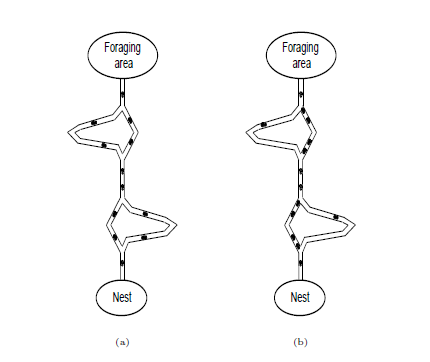
\includegraphics[scale=1]{img/01trasa.png}
\caption{Eksperyment podwójnego mostu. Obrazek do wykonania własnoręcznie Sytuacja a) przy rozpoczęciu eksperymentu, b) pod koniec trwania eksperymentu}
\label{fig:eksperyment}
\end{figure}
Kolejny eksperyment był analogiczny do pierwszego, jednak tym razem użyto mostów o różnych długości. Podczas obserwacji, początkowo mrówki również chodziły przypadkowo, korzystając z obu mostów. Po niedługim czasie zaczęto jednak dostrzegać rosnącą tendencję wyboru przez mrówki mostu krótszego. Działo się tak, ponieważ używając krótszej drogi, mrówka mogła przebyć ją w krótszym czasie, co skutkowało tym, że droga ta została użyta więcej razy, tak więc ślad feromonu był wyraźniejszy i częściej wzmacniany. To z kolei powodowało, że inne mrówki stając przed wyborem, również chętniej wybierały tę trasę, ponownie powodując swoiste sprzężenie zwrotne.
W feromonach więc pośrednio zawarte są informacje o przebiegu wcześniejszych tras, co pozwala na uwzględnienie tej wiedzy w
podjęciu decyzji dotyczącej wyboru trasy bieżącej. Jest to sposób prosty i wydajny, przez co wysoce atrakcyjny. Postanowiono więc wykorzystać go w algorytmice. W ten sposób powstał pierwszy koncept alorytmu mrówkowego.


\section{Cybernetyczne mrówki}\label{sec:wstepMrowki}
Po przeniesieniu rzeczywistości do świata zero-jedynkowego, kolonia mrówek zamiast pożywienia, potrafi wyszukać najkrótszą
ścieżkę, rozwiązać Problem Komiwojażera, czy też zaplanować optymalne trasy logistyczne dla firmy spedycyjnej. Są to problemy dużo bardziej rozbudowane, niż te postawione przed mrówkami żywymi, dlatego też zdecydowano się "udoskonalić" dzieło natury poprzez dodanie owadom kilku dodatkowych atrybutów. Jednym z nich jest \textbf{sposób rozmieszczania feromonu}. Jest on nanoszony dopiero "w drodze powrotnej", czyli, gdy cała trasa została przebyta. Oznacza to, że feromon może być rozprowadzony proporcjonalnie co do długości ścieżki, czyli że jest wyznacznikiem jakości znalezionej ścieżki. Także mrówka, dopiero szukając destynacji, nie natknie się na swój własny feromon, którego śladami wróci do gniazda. Jest to zmiana najważniejsza i występuje w praktycznie każdej wersji algorytmu. 
\newline 
Udoskonalony jest również \textbf{efekt zanikania (ewaporacji) feromonu}. W świecie komputerowym jest to proces dyskretny i kontrolowany, podczas gdy w przyrodzie zależeć może od szeregu czynników atmosferycznych, czy też losowych. 
\newline 
Cybernetyczne mrówki dysponują również \textbf{wiedzą a priori}. Wychodząc z mrowiska, dokładnie wiedzą, gdzie leży rozwiązanie, z każdym krokiem są świadome tego, czy do celu się zbliżają, czy też wręcz przeciwnie. Można to porównać do zapachu pożywienia, który może prowadzić mrówki w rzeczywistym świecie, jednak komputerowa informacja jest dużo bardziej pewna i precyzyjna. 
\newline
Każda cybernetyczna mrówka dysponuje również \textbf{wewnętrzną pamięcią}, którą może na różne sposoby wykorzystywać. Owad pamięta, którą drogą już szedł, które pola odwiedził i czy sąsiednie pole nie jest zablokowane. Wiedza ta pozwala na rozwinięcie szeregu ulepszeń.


\section{Podmiot badania}\label{sec:wstepPodmioti}
Badana cybernetycza kolonia mrówek, czyli technicznie rzecz ujmując Algorytm Mrówkowy, rozwiązywać będzie problem znalezienia najkrótszej ścieżki. Badania przeprowadzone będą w środowisku zapewniającym tworzenie oraz wczytanie mapy, ustawienie parametrów wejściowych oraz obserwację zarówno przebiegu, jak i wyniku algorytmu w interfejsie graficznym.





\chapter{Algorytm} \label{chap:algorytm}

\section{Opis problemu}\label{sec:algOpisProbl}
Rozpatrywany problem polega na poszukiwaniu najkrótszej ścieżki na zadanej mapie. Mapa jest zdyskretyzowana, podzielona na równe pola. Szukana ścieżka ma za zadanie łączyć dwa zadane punkty - start, którym w przyrodniczej analogii może być mrowisko, oraz destynację, którą reprezentować może źródło pożywienia. Na mapie znajdują się przeszkody. Poruszanie się po polach na których znajdują się przeszkody jest niemożliwe, zatem ścieżka musi takie pola omijać. Informacje o odległości każdego pola od destynacji są znane i traktowane jako wiedza \textit{a priori}.
\newline Poprzez pojęcie najkrótszej ścieżki rozumiany jest możliwie najmniejszy zbiór dostępnych pól łączących start z destynacją, takich, że każde pole sąsiaduje z polem kolejnym. 
 
\section{Zasada działania algorytmu}\label{sec:algorytmMetaH}
Kolonia mrówek (zbiór agentów), w określonej ilości ich osobników, równocześnie wyrusza z mrowiska i asynchronicznie porusza się w poszukiwaniu destynacji. Gdy wszystkie insekty osiągną cel, następuje oznaczenie każdej ze ścieżek feromonem. Każde dostępne pole na mapie ma do siebie przyporządkowaną określoną wartość feromonu. Wartości te będą miały wpływ na podejmowanie decyzji co do wyboru następnego kroku w kolejnych iteracjach mrówek. 
\newline 
Zarówno wiedza \textit{a priori}, jak i wartości feromonu składają się na prawdopodobieństwo wyboru danej ścieżki. Im wyższe prawdopodobieństwo, tym bardziej atrakcyjna droga. Nie jest to jednak nakaz. Mrówka może zdecydować się sugerowaną ścieżkę zignorować i wybrać inną, losową drogę. Dzięki takiej, czasami losowej, eksploracji szansa na znalezienie lepszej, krótszej trasy wzrasta.
\newline
 Mrówki pamiętają pola, które odwiedziły. Jest to kolejny atut, w jaki została wyposażona mrówka cybernetyczna. Informacja ta może zostać wykorzystana na wiele sposobów. W przypadku danego problemu, zapobiega ona wpadnięciu mrówki w oscylacje, czyli poruszanie się wciąż po tej samej zamkniętej pętli. Zjawisko podobne ma miejsce także w przyrodzie i znane jest pod nazwą "spirali śmierci mrówek" (ang. 'ant spiral of death' lub 'ant mill'). Występuje w momencie, gdy każda mrówka idzie śladem kolejnej, przy czym mrówka "pierwsza" podąża za tą "ostatnią". Są one wtedy odseperowane bardzo mocnym śladem feromonu od ucieczki, przez co w końcu umierają z wyczerpania.

\section{Metaheurystyka}\label{sec:algorytmMetaH}
Biorąc pod uwagę fakt, że mrówki poruszają się niezależnie od siebie, w czasie równoległym oraz każda z osobna jest w stanie znaleźć szukaną ścieżkę, wydawać by się mogło, że każda z nich równie dobrze poradziłaby sobie sama. Jest to błędny wniosek, siła tych insektów tkwi bowiem w mapie feromonowej, która to jest efektem pracy wielu. Być może mrówki "żyjące" w tej samej iteracji nie pomagają sobie wzajemnie, jednak ich doświadczenia pozwolą lepiej zaadaptować się kolejnym generacjom. Informacje zawarte w feromonach pośrednio zawierają więc dane o sukcesach i porażkach wcześniejszych pokoleń. Bazując na tym, mrówki z coraz mniejszym prawdopodobieństwem popełniać będą te same błędy. To wszystko po uwzględnieniu oczywiście informacji o odległościach każdego pola od destynacji, czyli wiedzy \textit{a priori}, zwanej także wiedzą heurystyczną. Wiedza ta jest bardzo często dostępna w tego typu problemach i pomaga wskazać mrówkom najlepiej rokujące ścieżki. Te dwie informacje powodują, że Algorytm Mrówkowy jest algorytmem \textit{metaheurystycznym}. Biorąc pod uwagę znaczenie łacińskiego wyrazu \textit{meta}, czyli "nad", w wolnym tłumaczeniu znaczy to, że mrówki, podczas swojego przeszukiwania mapy, dysponują nie tylko wiedzą heurystyczną, ale także czymś ponad to. Metaheurystyka nie zawsze gwarantuje znalezienie najbardziej optymalnego rozwiązania. Wiedza heurystyczna, historia porażek i sukcesów zawarta w śladach feromonowych oraz element stochastyczny, wszystko to razem pozwala jednak na odnalezienie szerokiego spektrum coraz to lepszych rozwiązań, z których każde kolejne ma szansę na bycie tym najlepszym.
\newline 
Feromony wraz z każdą iteracją poddane są zjawisku \textit{ewaporacji}. Jest to proces, w związku z którym intensywność feromonu maleje wraz z upływem czasu. Zapachy parują, tracąc na intensywności, dzieje się tak również w przyrodzie. W algorytmie skutkować to będzie unikaniem zbiegania do wyłącznie "utartych" ścieżek. Jest to swoisty element zapominania, który faworyzuje eksplorację terenów nowych. 
\newline 
Elementem metaheurystycznym jest także \textit{demon}. O demonie mówi się, gdy przedsięwzięte procedury nie mogłyby zostać wykonane przez pojedynczą mrówkę. Demon jest jednostką centralną. Posiada on wiedze globalną, niedostępną pojedynczemu agentowi danego algorytmu. Dzięki temu, może on stosować bardziej zaawansowane techniki, czy też metody analizy, prowadzące do rozwiązania problemu. Przykładem takiego postępowania może być decyzja o dodaniu pewnej ilości feromonu do tych pól odwiedzonych przez mrówkę w bieżącej iteracji, które jednocześnie należą do najlepszego globalnego rozwiązania, które zostało znalezione dotychczas. Innym praktycznym przykładem jest decyzja o odrzucaniu najgorszych znalezionych rozwiązań w  iteracji. Demon obserwuje wszystkie mrówki w danej iteracji i na tej podstawie potrafi zdecydować, która znalazła najgorsze rozwiązanie. Taka ścieżka nie zostanie oznaczona feromonem, albo zostanie oznaczona odpowiednio słabiej. Aktualizacje mapy feromonu, w które ingerował demon, nazywane są aktualizacjami  \textit{off-line}. Akcje demona nie są warunkiem koniecznym, a jedynie opcjonalnym. 
\newline Działania, które iteracyjnie wykonywane są przez Algorytm Mrówkowy w ramach metaheurystki, prezenują się następująco:
\begin{enumerate}
\item Aktywność mrówek
\begin{itemize}
\item poruszanie się celem znalezienia destynacji
\item aktualizacja feromonu na znalezionej ścieżce
\end{itemize}
\item Parowanie feromonu
\item Działania demona (opcjonalnie)
\end{enumerate}
Dokładna zasada działania każdego z tych punktów, jak również wzajemnego ich oddziaływania, nie jest wyspecyfikowana. Dzięki temu projektant algorytmu ma możliwość dopasowania go wedle potrzeb do sytuacji oraz rozwiązywanego problemu.

\section{Opis algorytmu}\label{sec:ralgorytmOpis}
Pojęcie Algorytmu Mrówkowego rozumiane jest na wiele sposobów. Odpowiednikiem tego pojęcia w języku angielskim jest "Ant Colony Algorithm" (w skrócie ACO), który tłumaczony dostłownie  oznacza "Algorytm Kolonii Mrówek". Tytułem tym oznaczana jest zarówno cała rodzina algorytmów, która bazuje na wspólnych "mrówczych" założeniach, jak również sztandarowy, klasyczny, oryginalny algorytm, który dał tejże rodzinie początek. Protoplasta ten nazywa się "Ant System" i stworzony został w 1991 roku przez Marco Dorigo. Od tamtego czasu, cieszący się wciąż rosnącą popularnością algorytm doczekał się wielu modyfikacji oraz rozgałęzień. Zazwyczaj jednak, używając nazwy "Algorytm Mrówkowy" (czy też ACO), ma się na myśli ów klasyczny "Ant System" i taka konwencja została przyjęta także w tej pracy.
\newline Już na samym początku istnienia algorytmu, zdefiniowano jego trzy wersje. Dwie z nich (\textit{ant-quantity} i \textit{ant-density}) zakładały aktualizację feromonów podczas budowania rozwiązania, trzecia (\textit{ant-cycle}) - po zdefiniowaniu całej ścieżki. Ta ostatnia już w fazie wstępnych tesów dawała znacznie lepsze wyniki od dwóch pozostałych, dlatego też skupiono się na niej. Z czasem dwie pierwsze całkowicie porzucono, a pozostały algorytm ochrzczony został mianem Algorytmu Mrówkowego.
\newline Jak już zostalo wspomniane, każde pole $i$ w rozpatrywanym problemie ma przyporządkowaną pewną wartość feromonu $\tau _{i}$. Wartość ta powstała podczas poprzednich iteracji oraz reprezentuje szansę na odniesienie sukcesu, po udaniu się na pole $i$ . Każda mrówka $k$, znajdując się na polu $h$, staje przy wyborze pola kolejnego. Decyzje swoją podejmuje biorąc pod uwagę zarówno $\tau_{i}$, jak również informację heurystyczną $\eta _{i}$ opisującą dane pole. Informacja ta w rozpatrywanym problemie zawiera odległość danego pola $\eta_{i}$ od destynacji. Im odległość większa - tym pole mniej atrakcyjne. Na podstawie tych informacji, mrówka potrafi znaczyć sobie wartość atrakcyjności $a_{i}$, jaką scharakteryzować można dane pole. Atrakcyjność ta jest zmienna, ponieważ w każdej iteracji zmienia się wartość feromonu $\tau_{i}$. Dlatego też oznaczyć ją można jako funkcję od czasu, czyli innymi słowy od iteracji $t$.  Wzór, z jakim jest ona wyliczana, prezentuje się następująco:
\newline
\begin{equation} \label{eq:atrakcyjnoscAS}
a_{hi}(t) = \frac{[ \tau_{i}(t)]^{\alpha} [\eta_{i}]^{\beta}}{ \sum_{l \in  N_{h} } [ \tau_{l}(t)]^{\alpha} [\eta_{l}]^{\beta}} \ \ \ \forall i \in N_{h}
\end{equation} 
\newline gdzie:
\begin{itemize}
\item $N_{h}$ - wszystkie dostępne pola leżące w sąsiedztwie pola $h$,
\item$\alpha, \beta$ - parametry wprowadzane do algorytmu, poprzez zmianę ich wartości można pośrednio kontrolować wpływ odpowiednio feromonu i wartości heurystycznej.
\end{itemize}
Wartość heurystyczna scharakteryzowana jest w następujący sposób:
\newline
\begin{equation}
\eta_{i} = \frac{1}{d_i}
\end{equation} 
gdzie $d_i$ jest odległością pola $i$ od destynacji.
\newline Na podstawie tak wyliczonej atrakcyjności, mrówka $k$ liczy prawdopodobieństwo udania się ze swojego pola $h$ na pole $i$. Wyraża ono się wzorem:
\newline
\begin{equation} \label{eq:prawAS}
p^k_{hi}(t) = \frac{ a_{hi}(t) }{ \sum_{l \in  N^k_{h}  } a_{hl}(t)  }
\end{equation} 
\newline gdzie $ N^k_{h}$ jest zbiorem dostępnych pól, które leżą w sąsiedztwie pola $h$ lecz zostały odwiedzone przez mrówkę $k$ najmniej razy. Warunek ten pozwala na uniknięcie wpadnięcia mrówki w pętlę. Zarówno zbiór $ N^k_{h}$ jak i informacje o ilości odwiedzin budowane są przy użyciu prywatnej pamięci mrówki $k$.
\newline Wpływ parametrów $\alpha$ oraz $\beta$ jest następujący:
\begin{itemize}
\item Gdy $\alpha = 0$, wpływ feromonów zostaje całkowicie wyłączony. Największe prawdopodobieństwo uzyskują wtedy pola, które znajdują się najbliżej celu. Wyłączenie informacji płynących z dodatkowych danych powoduje, że algorytm zachowuje się jak klasyczny algorytm chciwy. 
\item Gdy $\beta = 0$, tylko wpływ feromonów kieruje mrówkami. Z początku będą się one poruszać więc dość losowo, jednak już po kilku operacjach osiągną stagnację i poruszać się będą wciąż tą samą ścieżką.
\end{itemize}
Jak więc można zauważyć, dobór tych parametrów jest kluczowy dla powodzenia algorytmu. Należy dobierać je odpowiednio do badanej planszy oraz pamiętać o tym, że stosunek między nimi powinien zostać odpowiednio zachowany.
\newline Wzór ten zakłada niezerowe wartości feromonu, w innym przypadku zawsze zwracać będzie 0. Z tego powodu każde dostepne pole inicjalizowane jest niską wartością feromonu. Wartość ta jest równa dla każdego pola i dlatego w praktyce niczego nie zmienia.
\newline
Gdy wszystkie mrówki w danej iteracji osiągną cel, następuje rozmieszczenie feromonów na wybranych przez nie ścieżkach. Każda mrówka $k$ ma do dyspozycji pewną stałą ilość feromonu do rozdysponowania. Zmiana feromonu na danym polu $\Delta \tau^k_{i}(t)$ przedstawiana jest jako funkcja czasu, ponieważ zmienia się w każdej iteracji.
\begin{equation} 
\Delta \tau^k_{i}(t) = 
\begin{cases}
1/L^k(t)  \ \  , i \in T^k(t),
\\ 0 \ \ , i \notin T^k(t)
 \end{cases}
\end{equation} 
\newline gdzie:
\begin{itemize}
\item $T^k(t)$ - ścieżka znaleziona przez mrówkę $k$ w iteracji $t$,
\item $L^k(t) $ - dlugość ścieżki znalezionej przez mrówkę $k$ w iteracji $t$.
\end{itemize}
Wynika z tego, że aby dane pole zostało zaktualizowane z niezerową wartością feromonu, musi zawierać się w ścieżce mrówki $k$. Zyskiwany feromon jest natomiast stały dla każdego pola znajdującego się na trasie mrówki $k$ i jego wartość jest odwrotnie proporcjonalna do długości danej ścieżki, czyli do ilości pól, które w skład danej ścieżki wchodzą. Jasno z tego wynika, że im krótsza dana droga, tym więcej feromonu otrzymuje każde należące do niej pole. 
\newline W tym miejscu uwzględniany jest również efekt parowania feromonu. Ewaporacja feromonu określana jest przez stałą $\rho$ i przeprowadzana jest następująco:
\newline
\begin{equation} 
\tau_{i}(t)  \leftarrow (1-\rho)\tau_{i}(t) + \Delta\tau_{i}(t)
\end{equation} 
\newline \newline \newline 
\newline gdzie
\begin{itemize}
\item  $\Delta\tau_{i}(t) =  \sum^{m}_{k=1} \Delta \tau^k_{i}(t)$ ,
\item $m$ - ilość mrówek, ustalana przez użytkownika przy starcie algorytmu, stała w każdej iteracji.
\end{itemize}
Oznacza to, że ewaporacja ma miejsce tylko raz na iterację. Ze wzoru można wywnioskować również, że $\rho$ powinno zawierać się w przedziale $[0;1]$, przy czym jest ono proporcjonalnie odpowiedzialne za parowanie feromonu.


\section{Modyfikacje algorytmu}\label{sec:algMod}
Jak zostało wyżej wspomniane, rodzina algorytmów mrówkowych jest dość liczna. Dzieje się tak z powodu prostej stuktury oraz logiki w postępowaniu, którą zapewnia przyrodniczy pierwowzór. Poniżej opisane zostały najpopularniejsze odmiany tegoż algorytmu.
\begin{itemize}
\item \textbf{$AS_{rank}$}
\newline Rozszerzenie to zostało zaproponowane przez Bullnheimer'a, Hartl'a i Strauss'a. W tej wersji aktualizacja feromonu również odbywa się offline, jednak tutaj większą rolę odgrywa demon. Po pierwsze, szereguje on wszystkie mrówki $m$ na podstawie długości znalezionych przez nie ścieżek w danej iteracji $L_1(t),L_2(t),...,L_m(t)$. Następnie, zwiększenie poziomu feromonu nastepuje tylko dla $\sigma-1$ pierwszych ścieżek($\sigma$ jest parametrem ustalanym przez użytkownika), czyli ostatnie, najdłuższe trasy są odrzucane. Zwiększanie poziomu feromonu nie jest jednak równe, lecz proporcjonalne do jakości rozwiązania. Dodatkowo, w każdej iteracji zwiększana jest ilość feromonu na najlepszej ścieżce, która została dotychczas znaleziona. Jest to więc użycie opisanego wyżej Elitist AS, stworzonego przez Dorigo. Tak więc, biorąc pod uwagę wszystkie wyżej wymienione modyfikacje, zmiana wartości feromonu na polu $i$ prezentuje się następująco:
\newline
\begin{equation} \label{eq:ASrank}
\tau_{i}(t)  \leftarrow (1-\rho)\tau_{i}(t) + \Delta\tau_{i}^r(t) + \sigma \Delta \tau_i^+(t) 
\end{equation}
\newline
gdzie:
\newline
\begin{equation} \label{eq:ASrank1}
\Delta\tau_{i}^r(t) = \sum_{u=1}^{\sigma-1}\frac{(\sigma-u)}{L^u(t)}
\end{equation}
\begin{equation} \label{eq:ASrank2}
\Delta \tau_i^+(t) = \frac{1}{L^+(t)}
\end{equation}
\newline
gdzie $L^x$ oznaczają, jak we wcześniejszych przykładach, długość ścieżki $x$. Równania \ref{eq:ASrank1} oraz \ref{eq:ASrank2} zachodzą oczywiście w przypadkach, gdy dane pola $i$ należą do odpowiednio znalezionych ścieżek. W przeciwnym razie wartości $\Delta\tau_{i}^r(t)$ wynoszą 0, a jedynym składnikiem aktywnym w równaniu \ref{eq:ASrank} jest ewaporacja.
\newline Zaproponowane rozwiązanie nie sprzyja eksploracji (faworyzowanie najlepszego, jak dotąd, rozwiązania oraz odrzucenie najdłuższych ścieżek, czyli takich, na zbudowanie których mrówki musiały odwiedzić najwięcej pól, codostarczałoby informacji). Przy badaniach podczas tworzenia tejże wersji okazało się jednak, że znacznie poprawia jakość szukanych rozwiązań.
\item \textbf{$ACS$}
\newline Ant Colony System, czyli System Kolonii Mrówek, został wprowadzony przez Dorigo i Gambardella'ę w 1996 roku. Miał on na celu ulepszenie AS, które wtedy było skuteczne tylko przy niewielkich problemach. W tym podejściu zastosowano kilka zasadniczych zmian.
\newline Przede wszystkim, aktualizacja feromonu offline odbywa się tylko przy pomocy demona, który wzmacnia ślad feromonu tylko na najlepszym rozwiązaniu, znalezionym od początku działania programu. Do tego celu używany jest wzór:
\newline
\begin{equation}
\tau_{i}(t)  \leftarrow (1-\alpha)\tau_{i}(t) + \alpha \Delta \tau_i^+(t)
\end{equation}
\newline gdzie $\alpha$ jest wagą feromonu wpisywaną do algorytmu, natomiast $ \Delta \tau_i^+(t)$ jest zwyczajowo równe $ \frac{Q}{L^+(t)}$.
Kolejną zmianą jest reguła wyboru kolejnego pola, nazwana regułą \textit{pseudo-losowo-proporcjonalną}. Atrakcyjność pola wyliczana jest w taki sam sposób jak w przypadku AS, przy pomocy równania \ref{eq:atrakcyjnoscAS}. Do algorytmu wprowadzany jest kolejny parametr $q_0 \in [0,1]$. Następnie jednak losowana jest wartość $q$. Wartość ta jest losowa oraz inna dla każdej mrówki $k$ w każdej iteracji $i$. Jeśli spełniony jest warunek $q \leq q_0$, wtedy:
\newline
\begin{equation}
p^k_{hi}(t) = 
\begin{cases}
1\ jesli\ j\ =\ arg\ max\ A_{h} (t) 
\\ 0 \ w\ przeciwnym\ wypadku 
 \end{cases}
\end{equation}
\newline
gdzie $A_{h} (t) $ jest zbiorem atrakcyjności $a_{hi}(t)$ wszystkich dostępnych pól $i$ sąsiadujących z polem $h$.
\newline
Jeśli zaś $q>q_0$, wtedy prawdopodobieństwo jest przydzielane zgodnie ze wzorem \ref{eq:prawAS} z AS. Wynika zaś z tego, że gdy $q \leq q_0$, algorytm wybiera bezpieczne rozwiązanie, bazujące na heurystyce oraz historii zawartej w śladzie feromonowym. Dzięki dopasowywaniu $q_0$ można zatem modulować poziom eksploracji względem korzystania z dostępnej wiedzy.
\newline Największą zmianą jest jednak aktualizacja feromonu metodą online, krok po kroku, zwana też \textbf{lokalną regułą aktualizacji feromonu}. Tak więc w każdej iteracji, każda mrówka $k$ po przejściu na pole $i$ korzysta ze wzoru: 
\newline
\begin{equation}
\tau_{i}(t)  \leftarrow (1-\rho)\tau_{i}(t) + \rho \Delta \tau_i
\end{equation}
\newline
gdzie $\Delta \tau_i$ jest stała i zazwyczaj ustalana na bazie najkrótszej ścieżki znalezionej za pomocą Algorytmu Najbliższego Sąsiada. W rozważanym przypadku jednak dany algorytm byłby niemiarodajny (sprawdza się on w zagadnieniach typu Problem Komiwojażera), dlatego też, zdecydowano się wyliczyć tą wartość na podstawie wymiarów mapy. Zakładając, że cel, w przybliżeniu, znajduje się w przeciwnym kącie mapy, niż start, używana jest długość wektora przemieszczenia danej mrówki. Na tej podstawie, wzór wygląda następująco:
\begin{equation}
\Delta \tau_i = \Delta \tau_0 = \frac{Q}{\sqrt{(w_d - w_s)^2 + (h_d - h_s)^2}} 
\end{equation}
\newline
gdzie $w$ odpowiada szerokości, zaś $h$ - długości położenia punktów $s$ - startowego oraz $d$ - docelowego. Ustalenie wartości $\Delta \tau_0$ miało kluczowe znaczenie i przy opracowywaniu ACS przeprowadzono testy dla szeregu wartości. Powiązanie tej zmiennej ze znalezioną, względnie optymalną najkrótszą ścieżką, przyniosło najlepsze efekty.
\item \textbf{usuwanie pętli}
\newline Jest to prosta modyfikacja, stworzona podczas analizy badanego w tej pracy problemu. Jak zostało opisane w podrozdziale \ref{sec:algorytmMetaH}, mrówka przy wyborze kolejnego pola, najpierw kieruje się do tych dostępnych pól, które mają najniższą liczbę odwiedzin. Z tego powodu czasem dzieje się tak, że mrówka, wchodząc do przeszkody na kształt tunelu zakończonego brakiem przejścia, musi podążać nim aż do końca, mimo, że rozsądniejsze byłoby zawrócenie. Ścieżka zawierająca taką eksplorację tunelu jest z całą pewnością nieoptymalna, jak również ślad feromonu jest mniej klarowny, skoro został zużyty na próżno.
\begin{figure}[H]
\centering
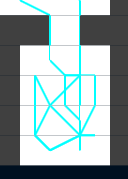
\includegraphics[scale=1]{img/02pomieszczenie.png}
\caption{Zachowanie mrówki przy pokonywaniu przeszkody typu "pomieszczenie".}
\label{fig:eksperyment}
\end{figure}
 Innymi słowy, jeśli mrówka musi wrócić do odwiedzanego wcześniej pola, to wszystkie pola na których przebywała pomiędzy tymi dwoma odwiedzinami nie przyniosły rozwiązania, można je więc uznać za zbędne. Celem wyłączenia takiego przebiegu wydarzeń stworzono usuwanie pętli. Po zbudowaniu całej ścieżki, jest ona przeszukiwana pod kątem pojawiania się pętli, które, w razie ich wystąpienia, są usuwane. 
\newline Rozwiązanie takie umożliwia szybsze znalezienie optymalnej ścieżki. Nie sprzyja ono jednak eksploracji mapy, co z kolei może mieć negatywny wpływ.
\end{itemize}






\end{document}